\documentclass[aspectratio=169,11pt]{beamer}
\usetheme{metropolis}
\usepackage{booktabs}
\usepackage{tikz}
\usetikzlibrary{positioning,fit,arrows.meta}
\graphicspath{{figures/}{../results/figures/}}

\title{How Much Downtime Do Replicas, Probes and Rolling Updates Remove?}
\subtitle{A measurement study on a local Kubernetes cluster --- SEN421 Topic 8, Part A}
\author{Ahmet Seyid Bilal Demircan \quad B2305.010146}
\institute{Istanbul Ayd\i n University --- SEN421 Cloud Architecture and Services}
\date{Fall 2026}

\begin{document}

\maketitle

% ---------------------------------------------------------------- 1
\begin{frame}{Problem and research question}
	\begin{itemize}
		\item Kubernetes promises \alert{self-healing} and \alert{zero-downtime updates}
		\item \dots but only if the workload is configured for it (replicas, probes, strategy)
	\end{itemize}
	\vspace{0.6em}
	\begin{block}{Question}
		How much user-visible downtime do a \textbf{pod failure} and a \textbf{version update} cause,
		how much is removed by \textbf{replicas + readiness probes} and \textbf{RollingUpdate},
		and how fast does the \textbf{HPA} react at 50\,\% vs 80\,\% CPU target --- at what cost?
	\end{block}
\end{frame}

% ---------------------------------------------------------------- 2
\begin{frame}{Setup}
	\begin{columns}[T]
		\column{0.55\textwidth}
		\centering
		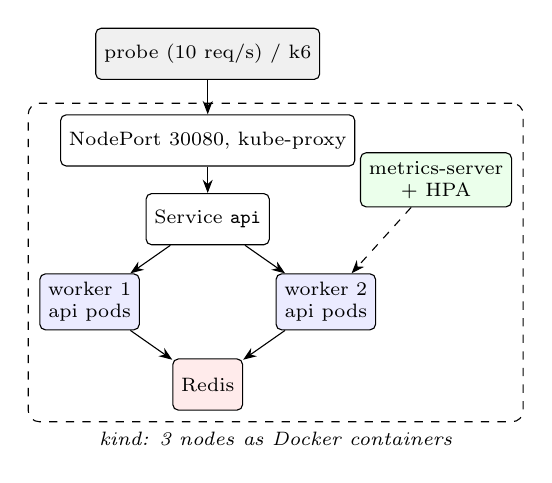
\begin{tikzpicture}[font=\scriptsize, >=Stealth,
			box/.style={draw, rounded corners=2pt, align=center, minimum height=0.65cm, inner sep=3pt, fill=white}]
			\node[box, fill=gray!12] (cl) at (0,0) {probe (10 req/s) / k6};
			\node[box] (np) at (0,-1.1) {NodePort 30080, kube-proxy};
			\node[box] (svc) at (0,-2.1) {Service \texttt{api}};
			\node[box, fill=blue!8] (w1) at (-1.5,-3.15) {worker 1\\api pods};
			\node[box, fill=blue!8] (w2) at (1.5,-3.15) {worker 2\\api pods};
			\node[box, fill=red!8] (rs) at (0,-4.2) {Redis};
			\node[box, fill=green!8] (hpa) at (2.9,-1.6) {metrics-server\\+ HPA};
			\draw[->] (cl) -- (np); \draw[->] (np) -- (svc);
			\draw[->] (svc) -- (w1); \draw[->] (svc) -- (w2);
			\draw[->] (w1) -- (rs); \draw[->] (w2) -- (rs);
			\draw[->, dashed] (hpa) -- (w2);
			\node[draw, dashed, rounded corners, fit=(np)(w1)(w2)(rs)(hpa), inner sep=4pt,
				label={[font=\scriptsize\itshape]below:kind: 3 nodes as Docker containers}] {};
		\end{tikzpicture}
		\column{0.45\textwidth}
		\small
		\begin{itemize}
			\item Flask API + Redis, 3 s warm-up
			\item kind, Kubernetes v1.37, 1 + 2 nodes
			\item Clients run \alert{inside} the kind network
			\item 3 runs per alternative, 18 runs
			\item Actual cost: \textbf{USD 0}
		\end{itemize}
	\end{columns}
\end{frame}

% ---------------------------------------------------------------- 3
\begin{frame}{Alternatives compared}
	\centering
	\begin{tabular}{lll}
		\toprule
		& \textbf{Alternative A} & \textbf{Alternative B} \\
		\midrule
		E1 pod failure & 1 replica, no probes & 3 replicas + readiness/liveness \\
		E2 update v1$\to$v2 & Recreate & RollingUpdate (surge 1, unavail.\ 0) \\
		E3 load (7 req/s) & HPA 80\,\% CPU & HPA 50\,\% CPU \\
		\bottomrule
	\end{tabular}
	\vspace{1em}

	\small Downtime = first to last failed request (non-200 or $>$1 s), seen by an external probe.
\end{frame}

% ---------------------------------------------------------------- 4
\begin{frame}{E1: pod failure}
	\begin{columns}[c]
		\column{0.58\textwidth}
		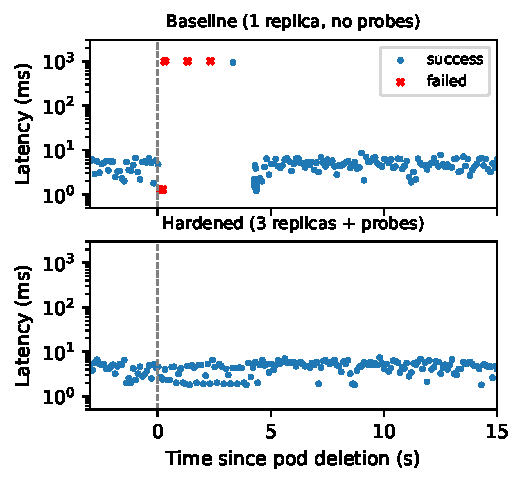
\includegraphics[width=\linewidth]{e1_timeline}
		\column{0.42\textwidth}
		\small
		\begin{tabular}{lcc}
			\toprule
			& Baseline & Hardened \\
			\midrule
			Failed req. & 5 & 0 \\
			Downtime & 3.21 s & 0 \\
			K8s Ready & 0.79 s & 4.42 s \\
			\bottomrule
		\end{tabular}
		\vspace{0.8em}

		\alert{Kubernetes said ``Ready'' after 0.8 s --- users saw errors for 3.2 s.}
	\end{columns}
\end{frame}

% ---------------------------------------------------------------- 5
\begin{frame}{E2: version update}
	\begin{columns}[c]
		\column{0.58\textwidth}
		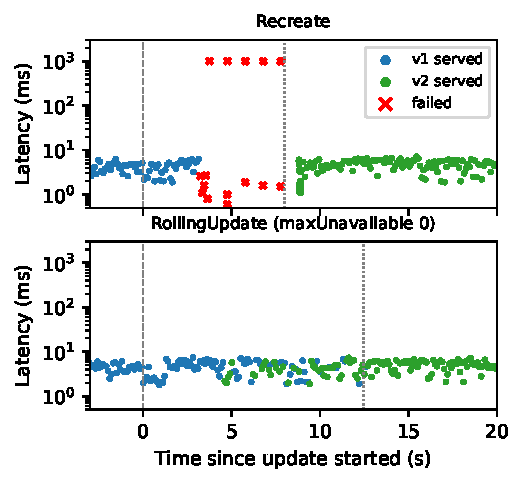
\includegraphics[width=\linewidth]{e2_timeline}
		\column{0.42\textwidth}
		\small
		\begin{tabular}{lcc}
			\toprule
			& Recreate & Rolling \\
			\midrule
			Rollout & 7.85 s & 12.41 s \\
			Failed req. & 14.3 & 0 \\
			Downtime & 5.37 s & 0 \\
			Two versions & 0 & 8.33 s \\
			\bottomrule
		\end{tabular}
		\vspace{0.8em}

		Zero downtime, but 58\,\% slower and v1 + v2 live together.
	\end{columns}
\end{frame}

% ---------------------------------------------------------------- 6
\begin{frame}{E3: autoscaling at 80\,\% vs 50\,\%}
	\begin{columns}[c]
		\column{0.58\textwidth}
		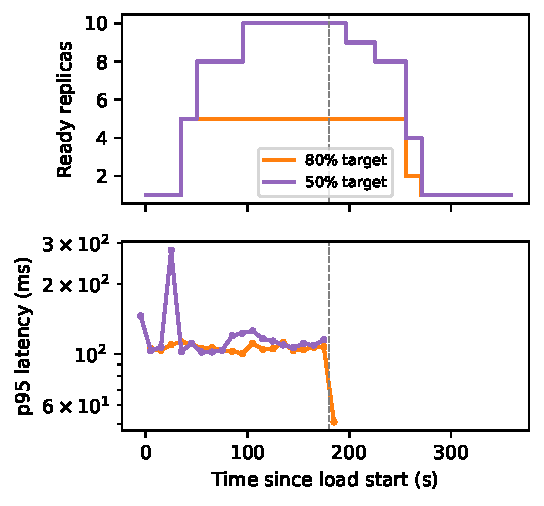
\includegraphics[width=\linewidth]{e3_hpa}
		\column{0.42\textwidth}
		\small
		\begin{tabular}{lcc}
			\toprule
			& 80\,\% & 50\,\% \\
			\midrule
			First scale-out & 35 s & 35 s \\
			Max replicas & 5.3 & 9.3 \\
			p95 latency & 118 ms & 112 ms \\
			Pod-seconds & 1323 & 2090 \\
			\bottomrule
		\end{tabular}
		\vspace{0.8em}

		50\,\%: +58\,\% pod time for the same latency.
	\end{columns}
\end{frame}

% ---------------------------------------------------------------- 7
\begin{frame}{Surprise: the autoscaler deadlock}
	\begin{itemize}
		\item First E3 attempt: 10 req/s = 500 m CPU = the pod's CPU limit
		\item Single pod overloaded $\to$ readiness probe failed $\to$ pod \alert{not ready}
		\item HPA ignores unready pods: \texttt{did not receive metrics for targeted pods}
		\item Stayed at \textbf{1 replica} for the whole run, 405--673 failed requests
	\end{itemize}
	\vspace{0.5em}
	\begin{block}{Lesson}
		\texttt{minReplicas} $\geq$ 2, realistic CPU requests, scale before saturation.
	\end{block}
\end{frame}

% ---------------------------------------------------------------- 8
\begin{frame}{Cost of availability (AKS estimate, Germany West Central)}
	\centering
	\begin{tabular}{lrr}
		\toprule
		USD / month & Baseline & Hardened \\
		\midrule
		Control plane (Free / Standard) & 0.00 & 73.00 \\
		B2s nodes (1 / 3) & 35.04 & 105.12 \\
		OS disks + public IP & 13.25 & 32.45 \\
		\midrule
		\textbf{Total} & \textbf{48.29} & \textbf{210.57} \\
		\bottomrule
	\end{tabular}
	\vspace{0.8em}

	\small Azure Retail Prices API, list prices, accessed 17 Nov 2026. Actual cost of this project: USD 0.\\
	Shared responsibility: AKS runs the control plane --- replicas, probes and HPA stay \alert{our} job.
\end{frame}

% ---------------------------------------------------------------- 9
\begin{frame}{Limitations}
	\begin{itemize}
		\item One physical host: pod deletion, not real machine or network failure
		\item Synthetic app and load, short runs, 3 repetitions
		\item List prices only (no discounts, data transfer, load balancer)
		\item Measurement path matters: Docker Desktop port forwarding turned 5 s into 20 s --- clients moved into the cluster network
	\end{itemize}
\end{frame}

% ---------------------------------------------------------------- 10
\begin{frame}{Conclusion}
	\begin{itemize}
		\item Replicas + readiness probes: pod failure \textbf{3.2 s $\to$ 0 s} downtime
		\item RollingUpdate: update \textbf{5.4 s $\to$ 0 s} downtime, but slower and mixed versions
		\item HPA 80\,\% was enough here; 50\,\% buys headroom at 58\,\% more pod time
		\item Hardened setup $\approx$ \textbf{4.4$\times$} the monthly cost on AKS
	\end{itemize}
	\vspace{0.5em}
	\begin{block}{Takeaway}
		Kubernetes gives the mechanisms --- availability comes from configuring them, and must be measured from the user's side.
	\end{block}
	\small Code and data: \url{https://github.com/demcan15/sen421-k8s-orchestration}
\end{frame}

\end{document}
